% Created 2019-06-29 六 04:55
% Intended LaTeX compiler: pdflatex
\documentclass[11pt]{article}
\usepackage[utf8]{inputenc}
\usepackage[T1]{fontenc}
\usepackage{graphicx}
\usepackage{grffile}
\usepackage{longtable}
\usepackage{wrapfig}
\usepackage{rotating}
\usepackage[normalem]{ulem}
\usepackage{amsmath}
\usepackage{textcomp}
\usepackage{amssymb}
\usepackage{capt-of}
\usepackage{hyperref}
\usepackage{minted}
\graphicspath{{../../images/ArtificialIntelligence/}}
% TIPS
% \substack{a\\b} for multiple lines text





% pdfplots will load xolor automatically without option
\usepackage[dvipsnames]{xcolor}

\usepackage{forest}
% two-line text in node by [two \\ lines]
% \begin{forest} qtree, [..] \end{forest}
\forestset{
  qtree/.style={
    baseline,
    for tree={
      parent anchor=south,
      child anchor=north,
      align=center,
      inner sep=1pt,
    }}}
%\usepackage{flexisym}
% load order of mathtools and mathabx, otherwise conflict overbrace

\usepackage{mathtools}
%\usepackage{fourier}
\usepackage{pgfplots}
\usepackage{amsthm, mathabx,  amsmath, commath}
\usepackage{amsfonts}

\usepackage{empheq}
\usepackage{tikz}
\usetikzlibrary{arrows.meta}
\usepackage[most]{tcolorbox}

\newtheorem{theorem}{Theorem}[section]
\newtheorem{definition}{Definition}[section]
\newtheorem{corollary}{Corollary}[section]
\newtheorem{example}{Example}[section]
\newtheorem{lemma}{Lemma}[section]
\newtheorem{proposition}{Proposition}[section]

\newcommand{\bl}[1] {\boldsymbol{#1}}
\newcommand{\Wt}[1] {\stackrel{\sim}{\smash{#1}\rule{0pt}{1.1ex}}}
\newcommand{\wt}[1] {\widetilde{#1}}


%For boxed texts in align, use Aboxed{}
%otherwise use boxed{}

\DeclareMathSymbol{\widehatsym}{\mathord}{largesymbols}{"62}
\newcommand\lowerwidehatsym{%
  \text{\smash{\raisebox{-1.3ex}{%
    $\widehatsym$}}}}
\newcommand\fixwidehat[1]{%
  \mathchoice
    {\accentset{\displaystyle\lowerwidehatsym}{#1}}
    {\accentset{\textstyle\lowerwidehatsym}{#1}}
    {\accentset{\scriptstyle\lowerwidehatsym}{#1}}
    {\accentset{\scriptscriptstyle\lowerwidehatsym}{#1}}
}

\usepackage{graphicx}
    
% text on arrow for xRightarrow
\makeatletter
%\newcommand{\xRightarrow}[2][]{\ext@arrow 0359\Rightarrowfill@{#1}{#2}}
\makeatother


\def \bx {\boldsymbol{x}}
\def \ba {\boldsymbol{a}}
\def \bI {\boldsymbol{I}}
\def \bt {\boldsymbol{t}}
\def \bb {\boldsymbol{b}}
\def \bA {\boldsymbol{A}}
\def \bX {\boldsymbol{X}}
\def \bu {\boldsymbol{u}}
\def \bS {\boldsymbol{S}}
\def \bZ {\boldsymbol{Z}}
\def \bz {\boldsymbol{z}}
\def \by {\boldsymbol{y}}
\def \bw {\boldsymbol{w}}
\def \bT {\boldsymbol{T}}
\def \bS {\boldsymbol{S}}
\def \bm {\boldsymbol{m}}
\def \bW {\boldsymbol{W}}
\def \bY {\boldsymbol{Y}}
\def \bH {\boldsymbol{H}}
\def \blambda {\boldsymbol{\lambda}}
\def \bPhi {\boldsymbol{\Phi}}
\def \btheta {\boldsymbol{\theta}}
\def \bmu {\boldsymbol{\mu}}
\def \bphi {\boldsymbol{\phi}}
\def \bSigma {\boldsymbol{\Sigma}}
\def \lb {\left\{}
\def \rb {\right\}}
\def \caln {\mathcal{N}}
\def \dissum {\displaystyle\Sigma}
\def \dispro {\displaystyle\prod}
\def \E {\mathbb{E}}
\def \Q {\mathbb{Q}}
\def \V {\mathbb{V}}
\def \R {\mathbb{R}}
\def \calq {\mathcal{Q}}
\def \calg {\mathcal{G}}
\def \caln {\mathcal{N}}
\def \calr {\mathcal{R}}
\def \calm {\mathcal{M}}
\def \calc {\mathcal{C}}
\def \bcup {\bigcup}

\author{wu}
\date{\today}
\title{Artificial Intelligence}
\hypersetup{
 pdfauthor={wu},
 pdftitle={Artificial Intelligence},
 pdfkeywords={},
 pdfsubject={},
 pdfcreator={Emacs 26.2 (Org mode 9.2.4)}, 
 pdflang={English}}
\begin{document}

\maketitle
\tableofcontents

\section{scope [28\%]}
\label{sec:org024efc6}
\begin{itemize}
\item[{$\boxtimes$}] uninformed search and informed search
\item[{$\boxtimes$}] adversarial search: minimax, evaluation functions, alpha-beta search,
stochasitc search
\item[{$\boxminus$}] Basic concept for Statistical Learning and modeling
\begin{itemize}
\item[{$\square$}] Probability Theory
\item[{$\square$}] Model selection
\item[{$\boxtimes$}] The curse of Dimensionality
\item[{$\square$}] Decision Theory
\item[{$\boxtimes$}] Information Theory
\item[{$\square$}] Probability Distribution
\end{itemize}
\item[{$\square$}] Supervised Learning
\begin{itemize}
\item[{$\square$}] Linear model for regression
\item[{$\square$}] Linear basis function models
\item[{$\square$}] Linear model for classification
\item[{$\square$}] Adaboosting
\end{itemize}
\item[{$\square$}] Unsupervised Learning
\begin{itemize}
\item[{$\square$}] K-means Clustering
\item[{$\square$}] GMM \& EM algorithm
\item[{$\square$}] Principal Component Analysis
\end{itemize}
\item[{$\square$}] Deep Learning
\begin{itemize}
\item[{$\square$}] Stochastic Gradient Descent
\item[{$\square$}] Backpropagation
\item[{$\square$}] Feedforward Neural Network
\item[{$\square$}] Convolutional Neural Networks
\item[{$\square$}] Deep learning in CV (localization)
\item[{$\square$}] Recurrent Neural Network (LSTM, GRU)
\end{itemize}
\item[{$\square$}] Reinforcement learning
\begin{itemize}
\item[{$\square$}] Reinforcement learning
\item[{$\square$}] Markov Decision Process
\item[{$\square$}] Value-based Optimization; Q-learning
\end{itemize}
\end{itemize}
\section{Basic concepts for filling in blanks or single choice [33\%]}
\label{sec:org8149850}
\begin{itemize}
\item[{$\boxtimes$}] Uninformed search (blind search)
\begin{itemize}
\item[{$\boxtimes$}] Problem definition, initial state, actions, transition model, goal
test, path cost, step cost, frontier (open list), loopy path, explored set
(closed set), tree-search, graph-search, queue, completeness, optimality,
time complexity, space complexity
\item[{$\boxtimes$}] Breadth-first search (BFS)
\item[{$\boxtimes$}] Depth-first search (DFS)
\item[{$\boxtimes$}] Uniform-cost search (UCS), Depth-limited search (DLS), iterative
deepening search (IDS)
\end{itemize}
\item[{$\boxtimes$}] informed (heuristic) search
\begin{itemize}
\item[{$\boxtimes$}] Heuristic function h(n), evaluation function f(n), path cost g(n)
\item[{$\boxtimes$}] Best-first search: use f(n) instead of g(n)
\item[{$\boxtimes$}] Greedy best-first search: f(n) = h(n)
\item[{$\boxtimes$}] A* search: f(n) = g(n) + h(n), it is identical to Uniform-Cost-Search
except that A* uses g+h instead of g
\item[{$\boxtimes$}] Conditions for A* optimality: Admissibility and Consistency

\textbf{Noteeeeeeeeee}
\end{itemize}
\item[{$\boxtimes$}] Adversarial search
\begin{itemize}
\item[{$\boxtimes$}] Minimax search: min node, max node, utility
\item[{$\boxtimes$}] Alpha-Beta Pruning Search: alpha value, beta value, pruning

\textbf{STARRRRRRRRRRRRRRRRR}
\end{itemize}
\item[{$\boxtimes$}] Uninformed search vs. informed search
\item[{$\square$}] common concepts
\begin{itemize}
\item[{$\square$}] train set, test set, validation set, S-fold cross-validation
\item[{$\square$}] model selection, model comparison
\item[{$\square$}] over-fitting, under-fitting, SSE error, RMS error, how to control over-fitting,
\item[{$\square$}] penalty term, regularization, shrinkage methods, curse of dimensionality,
\end{itemize}
\item[{$\square$}] probability theory
\begin{itemize}
\item[{$\square$}] marginal, joint distribution, conditional probability, PDF, CDF, expectation, variance,
covariance and their properties
\item[{$\square$}] i.i.d, MLE- Maximum Likelihood Estimation, MAPMaximum posterior, log
likelihood, Gaussian distribution, Mahalanobis distance,
\item[{$\square$}] independent parameters, conjugate prior, kernel density estimator, KNN density
estimator, KNN classifier,
\end{itemize}
\item[{$\boxminus$}] Information theory and decision theory
\begin{itemize}
\item[{$\boxtimes$}] entropy, cross entropy, relative entropy (Kullback-Leibler divergence, KL divergence),
mutual information
\item[{$\square$}] Naïve Bayes classifier, decision rule, reject option
\end{itemize}
\item[{$\square$}] Supervised learning
\item[{$\square$}] Regression: linear regression, linear basis function model, ridge regression,
stochastic gradient descent, weight decay, sparse model, lasso,
bias-variance tradeoff,
\item[{$\square$}] Classification: linear separable, decision regions, decision boundaries,
decision surfaces, 1-of-K code (one hot code), Least-squares approach,
Fisher’s linear discriminant, the perceptron algorithm of Rosenblatt, loss
function, hinge loss, The Fisher’s criterion, Generalized Rayleigh
quotient, Perceptron criterion, probabilistic generative model, logistic
sigmoid function, logit function, softmax function, probabilistic
discriminative model, logistic regression
\item[{$\square$}] Boosting: adaboost, committees, bagging, algorithm,
\item[{$\square$}] Unsupervised learning
\begin{itemize}
\item[{$\square$}] Clustering: partitional clustering, hierarchical clustering, k-means,
k-medoids, limitation, MoG, E-step, M-step
\item[{$\square$}] Dimensionality Reduction: latent factors, correlation, Pearson
correlation coefficient, correlation vs. independence, PCA, eigenface
\end{itemize}
\end{itemize}
\section{solving problems by search}
\label{sec:org495db00}
\textbf{problem-solving agent}
\begin{itemize}
\item \textbf{goal}
\item \textbf{goal information} is the 1st step in problem-solving, based on the
current situation and the agent’s performance measure
\item \textbf{problem formulation} is the process of deciding what actions and
states to consider, given a goal
\item \textbf{search}
\item \textbf{execution phase}
\end{itemize}


formulate—search—execution


type of search
\begin{itemize}
\item \textbf{uninformed search algorithms}

algorithms that are given no information about the problem other
than its definition. Although some of these algorithms can solve
any solvable problem, none of them can do so efficiently
\item \textbf{informed search algorithms}
\end{itemize}


The types of Problem-solving by Search
\begin{itemize}
\item Deterministic, fully observable

Agent knows exactly which state it will be in

solution is a sequence
\item non-observable

Agent may have no idea where it is

solution (if any) is a sequence
\item Nondeterministic and/or partially observable

percepts provide new information about current state

solution is a tree or policy

often interleave search, execution
\item Unknown state space
\end{itemize}


Some assumptions about environment
\begin{itemize}
\item \textbf{observable}
\item \textbf{discrete}: the environment is discrete
\item \textbf{known}: the agent knows which states are reached by each action
\item \textbf{deterministic}: each action has exactly one outcome
\end{itemize}


\textbf{Problem definition}
\begin{enumerate}
\item \textbf{Initial state}
\item \textbf{actions}
\item \textbf{Transition model}
\item \textbf{goal test}: determines whether a given state is a goal state
\item \textbf{path cost}: a function that assigns a numeric cost to each path
\end{enumerate}


A solution is an \textbf{action sequence}, so search algorithms work
by considering various possible action sequences.


Given a search tree, the set of all leaf nodes available for expansion at any
given point is called the \textbf{frontier(open list)}. \textbf{Search strategy}


queues: FIFO queue, LIFO queue (stack), priority queue


Measuring problem-solving performance: 
\begin{itemize}
\item completeness: Does it always find a solution
\item optimality: How long does it take?
\item time complexity
\item space complexity
\end{itemize}


\textbf{uninformd search}: Breadth-first search, Depth-first search


Strategies that know whether one non-goal state is “more promising” than
another are called \textbf{informed search} or \textbf{heuristic search} strategies

\subsection{uninformed search}
\label{sec:orgbc4a2ba}
Uniform-cost search: Instead of expanding the shallowest node, uniform-cost
search expands the node n with the lowest path cost g(n). This is done by
storing the frontier as a priority queue ordered by g(n)


DFS stack LIFO


Depth-limited search: 


Iterative deepening depth-first search: for depth = 0 to \(\infty\) do

\subsection{Informed search strategies}
\label{sec:orgbd1ab0d}
best-first search
\begin{itemize}
\item Best-first search is an instance of the general TREE-SEARCH or GRAPH-SEARCH
algorithm in which a node is selected for expansion based on an \textbf{evaluation
function} f(n)
\item The evaluation function is construed as a cost estimate, so the node with
the \textbf{lowest evaluation} is expanded first
\end{itemize}


\textbf{evaluation function} \(f\)
\begin{itemize}
\item Most best-first algorithms include as a component of f a \textbf{heuristic
function}, denoted h(n): \emph{estimated cost of the cheapest path from the state 
at node n to a goal state}
\item For now, we consider h(n) to be \textbf{arbitrary, nonnegative, problem-specific}
functions, with one constraint: if n is a goal node, then h(n)=0
\item \textbf{Greedy best-first search} : f(n) = h(n)
\end{itemize}


A* search:
f(n)=g(n)+h(n), h(n) the cost to get from the node to the goal


Conditions for optimality: \textbf{Admissibility} and Consistency
\begin{itemize}
\item f(n) = g(n) + h(n)
\item g(n) is the actual cost to reach n along the current path
\item h(n) is an \textbf{admissible heuristic} function: it never overestimates the cost
to reach the goal
\item So, f(n) never overestimates the true cost of a solution along the current
path through n
\end{itemize}


Conditions for optimality: Admissibility and \textbf{Consistency}
\begin{itemize}
\item h(n) ≤ c(n, a, n') + h(n')
\item for every node n and every successor n’ of n generated by any action a,
the estimated cost of reaching the goal from n is no greater than the step
cost of getting to n’ plus the estimated cost of reaching the goal from n
\end{itemize}


Properties of A* search
\begin{itemize}
\item The tree-search version of A* is optimal if h(n) is admissible
\item The graph-search version of A* is optimal if h(n) is consistent
\end{itemize}
\section{Adversarial search}
\label{sec:org5c2793b}

\subsection{Minimax search}
\label{sec:orgd4fe2bd}
\subsection{evaluation function}
\label{sec:orgf302591}
\subsection{Alpha-Beta Pruning Search}
\label{sec:orgfedd008}
\includegraphics[width=0.9\textwidth]{ABP}
\subsection{Monte-Carlo Tree Search}
\label{sec:org86d06df}

\section{Inference and Reasoning}
\label{sec:org59cc4a4}
\subsection{Propositional logic}
\label{sec:org7a7b19e}
\subsection{Predicate logic}
\label{sec:org396898c}
\subsection{First Order Inductive Learner}
\label{sec:org4056dfa}
\textbf{knowledge graph}: node = entity, edge = relation.
triplet (head entity, relation, tail entity)
\section{Statistical learning and modeling}
\label{sec:org94a38d0}
\subsection{Machine Learning: the concept}
\label{sec:org70f08e2}
\subsubsection{Example and concept}
\label{sec:org62d9dcb}
\begin{description}
\item[{Supervised learning problems}] applications in which the \textbf{training data} comprises examples of the input
vectors along with their corresponding \textbf{target vectors} are known

classification and regression
\item[{Unsupervised learning problems}] the training data consists of a set of input vectors X \textbf{without any
corresponding target values}

density estimation, clustering, hidden markov models
\item[{Reinforcement learning problem}] finding suitable actions to take in a given situation in order to
maximize a reward. Here the learning algorithm is not given examples of
optimal outputs, in contrast to supervised learning, but must instead
discover them by a process of trial and error. A general feature of
reinforcement learning is the trade-off between exploration and exploitation
\end{description}

types of machine learning
\begin{itemize}
\item supervised learning
\begin{itemize}
\item classification: the output is categorical or nominal variable
\item regression: the output is read-valued variable
\end{itemize}
\item unsupervised learning
\item semi-supervised learning
\item reinforcement learning
\item deep learning
\end{itemize}
\subsubsection{supervised learning: important concepts}
\label{sec:orgf704f90}
\begin{itemize}
\item Data: labeled instances \(<\bl{x}_i,\bl{y}>\)
\item features: attribute-value pairs which characterize each \(\bl{x}\)
\item learning a discrete function: \textbf{classification}
\item learning a continuous function: \textbf{regression}
\end{itemize}

\textbf{Classification} - A two-step process
\begin{itemize}
\item \textbf{model construction}
\item \textbf{model usage}
\end{itemize}

\textbf{regression}
\begin{itemize}
\item Example: price of a used car

\(\bl{x}\): car attributes. \(\bl{y}=g(\bl{x}\mid\bl{\theta})\): price. \(g\):
model. \(\theta\) parameter set.
\end{itemize}
\subsection{example: polynomial curve fitting}
\label{sec:orgb2056a9}
cross validation


SSE error(sum-of-square) \(E(\bl{w})=\frac{1}{2}\displaystyle\sum_{n=1}^N
   \lb y(x_n,\bl{w})-t_n\rb^2\)

RMS(root-mean-square) error \(E_{RMS}=\sqrt{2E(\bl{w}^*)/N}\)


How to control over-fitting
\begin{enumerate}
\item more train data
\item regularization
\item bayesian approach
\item cross-validation
\end{enumerate}


curse of dimensionality
\begin{itemize}
\item Extend polynomial curve fitting approach to deal with input spaces having
several variables. If we have D input variables, then a general polynomial
with coefficients up to order 3 would take the form:

\begin{equation*}
y(\bl{x},\bl{w})=w_0+\displaystyle\sum_{i=1}^Dw_ix_i+
\displaystyle\sum_{i=1}^D \displaystyle\sum_{j=1}^Dw_{ij}x_ix_j+
\displaystyle\sum_{i=1}^D \displaystyle\sum_{j=1}^D
\displaystyle\sum_{k=1}^Dw_{ijk}x_ix_jx_k
\end{equation*}
\end{itemize}
\subsection{probability theory review and notation}
\label{sec:org6ed1626}
rules of probability
\begin{itemize}
\item \textbf{sum rule} \(p(X)=\displaystyle\sum_Yp(X,Y)\)
\item \textbf{product rule} \(p(X,Y)=p(Y|X)p(X)\)
\end{itemize}

Bayes' Theorem: \(p(Y|X)=\frac{p(X|Y)p(Y)}{p(X)}\). Using sum rule
\(p(X)=\displaystyle\sum_Yp(X|Y)p(Y)\)

probability densities. 
\begin{align*}
p(x\in(a,b))&=\int_a^bp(x)dx\\
P(z)&=\int_{-\infty}^z p(x)dx\\
\int_{-\infty}^\infty p(x)dx&=1\quad p(x)\le0
\end{align*}
\(p(x)\) must satisfy two conditions
\begin{align*}
p(x)&\le 0\\
\int_{-\infty}^\infty p(x)dx&=1
\end{align*}


\textbf{expectation} \(\mathbb{E}[f]=
   \begin{cases}
   \displaystyle\sum_{x}p(x)f(x) & \text{discrete variables}\\
   \int p(x)f(x)dx & \text{continuous variables}
   \end{cases}\). In either cases,
\(\mathbb{E}[f]\approx\frac{1}{N}\displaystyle\sum_{n=1}^N f(x_n)\).
\textbf{conditional expectation}: \(\mathbb{E}_x[f| y]=\displaystyle\sum_xp(x| y)f(x)\).

The \textbf{variance} of \(f(x)\) is

\begin{align*}
var[f]&=\mathbb{E}[(f(x)-\mathbb{E}[f(x)])^2]\\
&=\mathbb{E}[f(x)^2-2f(x)\mathbb{E}[f(x)]+\mathbb{E}[f(x)]^2]\\
&=\mathbb{E}[f(x)^2]-\mathbb{E}[f(x)]^2
\end{align*}


The \textbf{covariance} is

\begin{align*}
cov[x,y]&=\mathbb{E}_{x,y}[(x-\mathbb{E}[x])(y-\mathbb{E}[y])]\\
&=\mathbb{E}_{x,y}[xy]-\mathbb{E}[x]\mathbb{E}[y]
\end{align*}


\begin{equation*}
\mathbb{V}[X]=\sigma^2_X=\E[(X-\E[X])^2]=\E[X^2]-\E[X]^2
\end{equation*}
\begin{equation*}
\V[\displaystyle\sum_{i=1}^nX_i]=\displaystyle\sum_{i=1}^n\V[X_i]+
\displaystyle\sum_{i\neq j}\text{Cov}[X_i,X_j]
\end{equation*}

\begin{align*}
&\text{Cov}[X,X]=\V[X]\\
&\text{Cov}[aX,bY]=ab\text{Cov}[X,Y]\\
&\text{Cov}[X+a,Y+b]=\text{Cov}[X,Y]
\end{align*}
\emph{the variance of the sum of two independent random variables is the sum of}
\emph{variance}. Given
\begin{center}
\begin{tabular}{c|c}
X & probability\\
\hline
\(x_1\) & \(p_1\)\\
\(\dots\) & \(\dots\)\\
\(x_n\) & \(p_n\)\\
\end{tabular}
\end{center}

\begin{center}
\begin{tabular}{c|c}
Y & probability\\
\hline
\(y_1\) & \(q_1\)\\
\(\dots\) & \(\dots\)\\
\(y_m\) & \(q_m\)\\
\end{tabular}
\end{center}
\begin{align*}
var(X+Y)=var(X)+var(Y)
\end{align*}

In case of two vectors of random variables \(\bl{x}\) and \(\bl{y}\), the
covariance is a matrix
\begin{align*}
cov[\bl{x},\bl{y}]&=\mathbb{E}_{\bl{x},\bl{y}}[(\bl{x}-\mathbb{E}[\bl{x}])(\bl{y}^T
-\mathbb{E}[\bl{y}^T])]\\
&=\mathbb{E}_{\bl{x},\bl{y}}[\bl{xy}^T]-\mathbb{E}[\bl{x}]\mathbb{E}[\bl{y}^T]
\end{align*}

\textbf{Bayesian probabilities}: \(P(A|B)=\frac{P(B|A)P(A)}{P(B)}\),
\(p(\mathcal{D})=\int p(\mathcal{D}|\bl{w})p(\bl{w})\text{d}\bl{w}\)
. For a data set 
\(\mathcal{D}=\{t_1,\dots,t_n\}\) and assumption \(w\),
\(p(w|\mathcal{D})=\frac{p(\mathcal{D}|w)p(w)}{p(\mathcal{D})}\). \(p(w)\) is
\textbf{prior probability}, \(p(\mathcal{D}|w)\) is \textbf{likelihood} (the probability
\(\mathcal{D}\) happens). Hence 
\begin{equation*}
\text{posterior}\propto\text{likelihood}\times\text{prior}
\end{equation*}

\textbf{Gaussian distribution}.
\begin{equation*}
\mathcal{N}(x|\mu,\sigma^2)=\frac{1}{(2\pi\sigma^2)^{1/2}}\exp\left\{
-\frac{1}{2\sigma^2}(x-\mu)^2\right\}
\end{equation*}
\(\mu\) is called \textbf{mean}, \(\sigma^2\) is called \textbf{variance}, \(\sigma\) \textbf{standard
deviation}, \(\beta=1/\sigma^2\) \textbf{precision}
\begin{align*}
\mathbb{E}[x]&=\int_{-\infty}^\infty\mathcal{N}(x|\mu,\sigma^2)xdx=\mu\\
\mathbb{E}[x^2]&=\int_{-\infty}^\infty\mathcal{N}(x|\mu,\sigma^2)x^2dx=\mu^2
+\sigma^2\\
var[x]&=\mathbb{E}[x^2]-\mathbb{E}[x]^2=\sigma^2\\
\end{align*}
For \$D\$-dimensional vector \(\bl{x}\) of continuous variables
\begin{equation*}
\mathcal{N}(\bl{x}|\bl{\mu},\bl{\Sigma})=\frac{1}{(2\pi)^{D/2}}\frac{1}
{\abs{\bl{\Sigma}}^{1/2}}\exp\left\{-\frac{1}{2}(\bl{x}-\bl{\mu})^T
\bl{\Sigma^{-1}}(\bl{x}-\bl{\mu})\right\}
\end{equation*}

To determine values for the unknown parameters given \(\mu\) and \(\sigma^2\) by
maximizing the likelihood function. Use log.
\begin{align*}
P(\bl{X}|\mu,\sigma^2)&=\displaystyle\prod_{n=1}^N\mathcal{N}(x_n|\mu,\sigma^2)\\
\Rightarrow \ln P(\bl{X}|\mu,\sigma^2)&=-\frac{1}{2\sigma^2}
\displaystyle\sum_{n=1}^N(x_n-\mu)^2-\frac{N}{2}\ln\sigma^2-\frac{N}{2}\ln(2\pi)\\
\end{align*}
Hence \(\mu_{ML}=\frac{1}{N}\displaystyle\sum_{n=1}^Nx_n\),
\(\sigma^2_{ML}=\frac{1}{N}\displaystyle\sum_{n=1}^N(x_n-\mu_{ML})^2\) by
partial derivative.
\(\E[\sigma_{ML}^2]=(\frac{N-1}{N})\sigma^2\)

Maximum likelihood estimator for mean is unbiased, that
  is, \(\mathbb{E}(\mu_{ML})=\mu\). Maximum likelihood estimator for variance is
  biased. \(\mathbb{E}(\sigma_{ML}^2)=\mathbb{E}(x^2)-\mathbb{E}(\mu_{ML}^2)=
   \frac{N-1}{N}\sigma_x^2\)
\subsection{information theory}
\label{sec:org766595a}
\textbf{entropy}: measuring uncertainty of a random variable \(X\).
\(H(X)=H(p)=-\displaystyle\sum_{x\in\Omega}p(x)\log p(x)\) where \(\Omega\) is
all possible values and define \(0\log0=0,\log=\log_2\)

\(H(X)=\displaystyle\sum_{x\in\Omega}p(x)\log_2\frac{1}{p(x)}=
   E(\log_2\frac{1}{p(x)})\). And "information of \(x\)"​="\#bits to code \(x\)"​=\(-\log
   p(x)\)

\textbf{Kullback-Leibler divergence}: comparing two distributions
\(D_{KL}(p||q)=H(p,q)-H(p)=-\int p(\bl{x})\ln\lb \frac{q(\bl{x})}{p(\bl{x})}d\bl{x}\)

\url{https://www.youtube.com/watch?v=ErfnhcEV1O8}


\textbf{mutual information}
\(I[\bl{x},\bl{y}]=\text{KL}(p(\bl{x},\bl{y})||p(\bl{x})p(\bl{y}))=H(\bl{y})-H[\bl{y}|\bl{x}]\)
\subsection{The gaussian distribution}
\label{sec:org3ddb9b9}
\begin{align*}
\Delta^2&=(x-\mu)^T\Sigma^{-1}(x-\mu)\\
&=(x-\mu)^TU\Lambda^{-1}U^T(x-\mu)\\
&=(U^T(x-\mu))^T\Lambda^{-1}(U^T(x-\mu))=y^T\Lambda^{-1}y
\end{align*}


\(\Sigma u_i=\lambda_i u_i\) where \(i=i,\dots,D\).
\begin{equation*}
\Sigma U=\Sigma(u_1,\dots,u_D)=(u_1,\dots,u_D)
\begin{pmatrix}
\lambda_1 & \dots & 0\\
\vdots & \ddots & \vdots\\
0&\dots &\lambda_D
\end{pmatrix}=U\Lambda
\end{equation*}

\(\forall i,j\in\lb 1,\dots,D\rb\),
\begin{equation*}
u_i^Tu_j=I_{ij}=
\begin{cases}
1&\text{if } i=j\\
0%\text{otherwise}
\end{cases}
\end{equation*}

\begin{equation*}
U^TU=I
\end{equation*}
So \(U\) is orthogonal, \(\Sigma UU^T=U\Lambda
   U^T=\displaystyle\sum_{i=1}^D\lambda_i u_iu_i^T\), and \(\Sigma^T=U\Lambda^{-1}U^T\)

\begin{equation*}
\Delta^2=\bl{y}^T\Lambda^{-1}\bl{y}\xrightarrow{y_i=\bl{u}_i^T(\bl{x}-\bl{\mu})}
\displaystyle\sum_{i=1}^D\frac{y_i^2}{\lambda_i}
\end{equation*}


GIven a square matrix \(A\in\R^{n\times n},x\in\R^n\), \(x^TAx\) is called a
\textbf{quadratic form}
\begin{equation*}
x^TAx=\displaystyle\sum_{i=1}^nx_i(Ax)_i_=\displaystyle\sum_{i=1}^n x_i
(\displaystyle\sum_{j=1}^nA_{ij}x_j)=\displaystyle\sum_{i=1}^n
\displaystyle\sum_{j=1}^nA_{ij}x_ix_j
\end{equation*}

\begin{equation*}
x^TAx=(x^TAx)^T=x^T(1/2A+1/2A^T)x
\end{equation*}
\subsection{model selection}
\label{sec:org8c9ba1e}
\textbf{cross-validation}
\includegraphics[width=100mm]{CrossValidation}

split training data into \textbf{training set} and \textbf{validation set}. Train different
models on training set and choose model with minimum error on validation set.
\subsection{decision theory}
\label{sec:orgc541245}
Suppose we have an input vector \(\bl{x}\) together with a corresponding vector
\(\bl{t}\) of target variables and our goal is to predict \(\bl{t}\) given new
value for \(\bl{x}\). The joint probability distribution \(p(\bl{x},\bl{t})\)
provides a complete summary of the uncertainty with these variables
\section{Statistical learning and modeling - Supervised learning}
\label{sec:org086ebdc}
\subsection{Basic concepts}
\label{sec:orgde9d247}
\begin{itemize}
\item \textbf{Linearly separable}
\begin{itemize}
\item decision regions:

input space is divided into several regions
\item decision boundaries:
\begin{itemize}
\item under linear models, it's a linear function
\item (D-1)-dimensional hyper-plane within the D-dimensional input space
\end{itemize}
\end{itemize}
\item \textbf{representation of class labels}
\begin{itemize}
\item Two classes K = 2
\item K classes
\begin{itemize}
\item 1-of-K coding scheme \(\bl{t}=(0,0,1,0,0)^T\)
\end{itemize}
\item Predict discrete class labels
\begin{itemize}
\item linear model prediction \(y(\bl{x})=\bl{w}^T\bl{x}+w_0\)
w: weight vector, w\textsubscript{0} bias/threshold
\item nonlinear function \(f(.):R\to(0,1)\)
\item generalized linear models
\(y(\bl{x})=f(\bl{w}^T\bl{x}+w_0)\)
f:activation function
\item dicision surface
\(y(\bl{x})=\text{constant}\to \bl{w}^T\bl{x}+w_0=\text{constant}\)
\end{itemize}
\end{itemize}
\item \textbf{Three classification approaches}
\begin{itemize}
\item discriminant function
\begin{itemize}
\item least squares approach
\item fisher's linear discriminant
\item the perceptron algorithm of rosenblatt
\end{itemize}
\item use discriminant functions directly and don't compute probabilities

Given discriminant functions \(f_1(\bl{x}),\dots,f_K(\bl{x})\). Classify
\(\bl{x}\) as class \(\mathcal{C}_k\) iff \(f_k(\bl{x})>f_j(\bl{x}),\forall
       j\neq k\)

\begin{itemize}
\item \textbf{least-squares approach}: making the model predictions as close as
possible to a set of target values
\item \textbf{fisher's linear discriminant}: maximum class separation in the ouput
space
\item \textbf{the perceptron algorithm of rosenblatt}
\end{itemize}
\item generative approach
\begin{itemize}
\item model the class-conditional densities and the class priors
\item compute posterior probabilities through Bayes's theorem

\(\underbrace{p(\mathcal{C}_k|\bl{x})}_\text{posterior for class}=
         \frac{\overbrace{p(\bl{x}|\mathcal{C}_k)}^\text{class conditional density}
         \overbrace{p(\mathcal{C}_k)}^\text{class prior}}{p(\bl{x})}=
         \frac{p(\bl{x}|\mathcal{C}_k)p(\mathcal{C}_k)}{\sum_{j}p(\bl{x}|\mathcal{C}_j)
         p(\mathcal{C}_j)}\)
\end{itemize}
\end{itemize}
\end{itemize}
\subsection{discriminant functions}
\label{sec:org81771dd}
\subsubsection{Two classes}
\label{sec:org8fe285b}
\begin{itemize}
\item Linear discriminant function \(y(\bl{x})=\bl{w}^T\bl{x}+w_0\)
\begin{itemize}
\item Dicision surface \(\Omega:y(\bl{x})=0\)
\item the normal distant from the origin to the dicision surface
\(\frac{\bl{w}^T\bl{x}}{\norm{\bl{w}}}=-\frac{w_0}{\norm{\bl{w}}}\)
\item if \(x_A,x_B\) lie on the decision surface \(y(\bl{x}_A)=y(\bl{x}_B)=0\),
then \(\bl{w}^T(\bl{x}_A-\bl{x}_B)=0\). hence w is orthogonal to every
vector lying within Ω. \(\frac{\bl{w}}{\norm{\bl{w}}}\) is the normal
vector of Ω

\item \(\bl{x}=\bl{x}_\perp+r\frac{\bl{w}}{\norm{\bl{w}}}\) hence
\(r=\frac{y(\bl{x})}{\norm{\bl{w}}}\). \(y(\bl{x}_\perp)=0\to
        \bl{w}^T\bl{x}=-w_0+r\frac{\bl{w}^T\bl{w}}{\norm{\bl{w}}}\)
\item \(\tilde{\bl{w}}=(w_0,\bl{w}), \tilde{\bl{x}}=(x_0,\bl{x}),
        y(\bl{x})=\tilde{\bl{w}}^T\tilde{\bl{x}}\)
\end{itemize}
\end{itemize}
\subsubsection{K-class}
\label{sec:org066d8c3}
\begin{itemize}
\item One-versus-the-rest classifier
K - 1 classifiers each of which solves a two-class problem
\item One-versus-one classifier
K(K-1)/2 binary discriminant functions
\item single K-class discriminant comprising K linear functions
\(y_k(\bl{x})=\bl{w}_k^T\bl{x}+w_{k_0}\)
\begin{itemize}
\item assigning a point x to class \(\mathcal{C}_k\) if
\(y_k(\bl{x}>y_j(\bl{x}))\) for all j≠k
\item dicision boundary between class \(\mathcal{C}_k, \mathcal{C}_j\) is given
\(y_k(\bl{x})=y_j(\bl{x})\to
        (\bl{w}_k-\bl{w}_j)^T\bl{x}+(w_{k_0}-w_{j_0})=0\)
\item \(\mathcal{R}_k\) is singly connected convex
\item \(\hat{\bl{x}}=\lambda\bl{x}_A+(1-\lambda)\bl{x}_B\) where \(0\le\lambda\le
        1\), \(y_k(\hat{\bl{x}})=\lambda y_k(\bl{x}_A)+(1-\lambda)y_k(\bl{x}_B)\)
and hence \(\hat{x}\) also lies inside \(\mathcal{R}_k\)
\end{itemize}
\end{itemize}
\subsubsection{Learning the parameters of linear discriminant functions}
\label{sec:org615308f}
\begin{enumerate}
\item Linear basis function models
\label{sec:org94224f4}
\textbf{linear regression}:
\(y(\bl{x},\bl{w})=w_0+w_1x_1+\dots+w_Dx_D=\bl{w}^T\bl{x}\).

For nonlinear functions \(\phi_j\),
\(y(\bl{x},\bl{w})=w_0+\displaystyle\sum_{j=1}^{M-1}
     w_j\phi_j(\bl{x})=\bl{w}^T\bl{\phi(\bl{x})}\) where \(\phi_j(\bl{x})\) are
\textbf{basis functions} 
\item \textbf{parameter optimization via maximum likelihood}
\label{sec:org331bad0}

Assume target variable \(t\) is given by a deterministic function
\(y(\bl{x},\bl{w})\) with additive Gaussian noice so that
\(t=y(\bl{x},\bl{w})+\epsilon\) where \(\epsilon\) is a zero mean Gaussian
random variable with precision \(\beta\), hence we can write
\begin{equation*}
p(t|\bl{x},\bl{w},\beta)=\mathcal{N}(t|y(\bl{x},\bl{w}),\beta^{-1})
\end{equation*}
and \(\mathbb{E}(t|\bl{x})=\int tp(t|\bl{x})dt=y(\bl{x},\bl{w})\)

For data set \(\bl{X}=\{\bl{x}_1,\dots,\bl{x}_n\},\bl{t}=(t_1,\dots,t_n)^T\),
\(p(\bl{t}|\bl{X},\bl{w},\beta)=\displaystyle\prod_{n=1}^N\mathcal{N}(t_n|
     \bl{w}^T\bl{\phi}(\bl{x}_n),\beta^{-1})\)

\(\ln p(\bl{t}|\bl{w},\beta)=\displaystyle\sum_{n=1}^N\ln\mathcal{N}(t_n|
     \bl{w}^T\bl{\phi}(\bl{x}_n),\beta^{-1})=\frac{N}{2}\ln\beta-\frac{N}{2}\ln(2\pi)-
     \beta E_D(\bl{w})\)

\(E_D(\bl{w})=\frac{1}{2}\displaystyle\sum_{n=1}^N
     \left\{t_n-\bl{w}^T\bl{\phi}(\bl{x}_n)\right\}^2=
     \frac{1}{2}\norm{t-\Phi\bl{w}}\) is sum-of-squares error function

solve \(\bl{w}\) by maximum likelihood.
\begin{equation*}
\nabla\ln p(\bl{t}|\bl{w},\beta)=\displaystyle\sum_{n=1}^N
\left\{t_n-\bl{w}^T\bl{\phi}(\bl{x}_n)\right\}\phi(\bl{x}_n)^T
\end{equation*}
\begin{equation*}
0=\displaystyle\sum_{n=1}^N t_n\bl{\phi}(\bl{x}_n)^T-\bl{w}^T
(\displaystyle\sum_{n=1}^N\bl{\phi}(\bl{x}_n)\bl{\phi}(\bl{x}_n)^T)
\end{equation*}
Hence we get
\begin{equation*}
\bl{w}_{ML}=(\bl{\Phi}^T\bl{\Phi})^{-1}\bl{\Phi}^T\bl{t}
\end{equation*}
\(\Phi\) is \textbf{design matrix}.
\[
\Phi=\begin{pmatrix}
 \phi_0(\bl{x}_1) & \phi_1(\bl{x}_1) & \dots & \phi_{M-1}(\bl{x}_1) \\
 \phi_0(\bl{x}_2) & \phi_1(\bl{x}_2) & \dots & \phi_{M-1}(\bl{x}_2) \\
 \vdots & \vdots & \ddots & \vdots \\
 \phi_0(\bl{x}_N) & \phi_1(\bl{x}_N) & \dots & \phi_{M-1}(\bl{x}_N) \\
\end{pmatrix}
\]

For bias parameter \(w_0\).
\(E_D(\bl{w})=\frac{1}{2}\displaystyle\sum_{n=1}^N 
     \{t_n-w_0-\displaystyle\sum_{j=1}^{M-1}w_j\phi_j(\bl{x}_n)\}^2\). Hence
\(w_0=\bar{t}-\displaystyle\sum_{j=1}^{M-1}w_j\bar{\phi_j}\),
\(\bar{t}=\frac{1}{N}\displaystyle\sum_{n=1}^Nt_n\),
\(\bar{\phi_j}=\frac{1}{N}\displaystyle\sum_{n=1}^N\phi_j(\bl{x}_n)\).

\(frac{N}{2\beta}=E_D(\bl{w})\). \(\frac{1}{\beta_{ML}}=
     \frac{1}{N}\displaystyle\sum_{n=1}^N\left\{t_n-\bl{w}^T_{ML}
     \bl{\phi}(\bl{x}_n)\right\}^2\)
\item Least-squares approach
\label{sec:org46201a8}
\begin{itemize}
\item Problem
\begin{itemize}
\item Each class \(\mathcal{C}_k\) is described by its own linear model 
\(y_k(\bl{x})=\bl{w}_k^T\bl{x}+w_{k0}\)
\item group together: \(y(\bl{x})=\widetilde{\bl{W}}^T\tilde{\bl{x}}\),
\(\tilde{\bl{w}}_k=(w_{k0},\bl{w}_k^T)^T\), \(\tilde{\bl{x}}=(1,\bl{x}^T)^T\)
\end{itemize}
\item Learning
\begin{itemize}
\item minimizing SSE function sum-of-squares
\(SSE=\displaystyle\sum_{i=1}^n(y_i-f(x_i))^2\)
\(E_D(\widetilde{\bl{W}})=1/2\text{Tr}\{(\bl{\widetilde{X}\widetilde{W}-T})^T 
         (\bl{\widetilde{X}\widetilde{W}-T})\}\)

\(\bl{\widetilde{W}}=(\bl{\widetilde{X}}^T\bl{\widetilde{X}})^{-1}\bl{\widetilde{X}}^T\bl{T}\)
\end{itemize}
\end{itemize}
\item fisher's linear discriminant
\label{sec:org86da102}

\includegraphics[width=100mm]{Fisher}

from the view of dimensionality reduction
\(y\ge -w_0\) as class \(\mathcal{C}_1\)

\(m_1=\frac{1}{N_1}\displaystyle\sum_{n\in\mathcal{C}_1}x_n, 
     m_2=\frac{1}{N_2}\displaystyle\sum_{n\in\mathcal{C}_2}x_n
     \xrightarrow{y=\bl{w}^T\bl{x}} m_2-m_1=\bl{w}^T(\bl{m}_2-\bl{m}_1)\)
\item the perceptron algorithm of rosenblatt
\label{sec:orgdce6e82}
\end{enumerate}
\subsection{probalibilistic generative models}
\label{sec:org3cc23bd}
A probabilistic view of classification from simple assumptions about the
distribution of the data

\begin{align*}
p(\mathcal{C}_1|\bl{x})&=\frac{p(\bl{x}|\mathcal{C}_1)p(\mathcal{C}_1)}
{p(\bl{x}|\mathcal{C}_1)p(\mathcal{C}_1)+p(\bl{x}|\mathcal{C}_2)p(\mathcal{C}_2)}\\
&=\frac{1}{1+\exp(-a)}=\sigma(a)
\end{align*}
where 
\begin{equation*}
a=\ln\frac{p(\bl{x}|\mathcal{C}_1)p(\mathcal{C}_1)}
{p(\bl{x}|\mathcal{C}_2)p(\mathcal{C}_2)}
\end{equation*}
and \(\sigma(a)\) is the \textbf{logistic sigmoid} function defined by
\begin{equation*}
\sigma(a)=\frac{1}{1+\exp(-a)}
\end{equation*}
and \(\sigma(-a)=1-\sigma(a)\), its inverse is \textbf{logit} function
\begin{equation*}
a=\ln(\frac{\sigma}{1-\sigma})
\end{equation*}

For case of \(K > 2\) classes, we have the following \textbf{multi-class generalization}
\begin{equation*}
p(\mathcal{C}_k|\bl{x})=\frac{p(\bl{x}|\mathcal{C}_k)p(\mathcal{C}_k)}
{\sum_jp(\bl{x}|\mathcal{C}_j)p(\mathcal{C}_j)}=\frac{\exp(a_k)}{\sum_j\exp(a_j)},
a_k=\ln\left[p(\bl{x}|\mathcal{C}_k)p(\mathcal{C}_k)\right]
\end{equation*}
The \textbf{normalized exponential} is known as the \textbf{softmax function} as it represents
a \emph{smoothed version of the max function}
\begin{equation*}
\text{if } a_k\ll a_j,\forall j\neq k,\text{then } p(\mathcal{C}_k|\bl{x})\approx 1,
p(\mathcal{C}_j|\bl{x})\approx 0
\end{equation*}

For \textbf{continuous inputs}, assume
\begin{equation*}
p(\bl{x}|\mathcal{C}_k)=\frac{1}{(2\pi)^{D/2}}\frac{1}
{\abs{\bl{\Sigma}}^{1/2}}\exp\left\{-\frac{1}{2}(\bl{x}-\bl{\mu}_k)^T
\bl{\Sigma^{-1}}(\bl{x}-\bl{\mu}_k)\right\}
\end{equation*}
\begin{enumerate}
\item 2 classes
\begin{align*}
p(\mathcal{C}_1|\bl{x})&=\sigma(\bl{w}^T\bl{x}+w_0)\\
\bl{w}&=\bl{\Sigma}^{-1}(\bl{\mu}_1-\bl{\mu}_2)\\
w_0&=-\frac{1}{2}\bl{\mu}_1^T\bl{\Sigma}^{-1}\bl{\mu}_1+
\frac{1}{2}\bl{\mu}_2^T\bl{\Sigma}^{-1}\bl{\mu}_2+\ln\frac{p(\mathcal{C}_1)}
{p(\mathcal{C}_2)}\\
\end{align*}
\item K classes
\begin{align*}
a_k(\bl{x})&=\bl{w}_k^T\bl{x}+w_{k0}\\
\bl{w}_k&=\bl{\Sigma}^{-1}\bl{\mu}_k\\
w_{k0}&=-\frac{1}{2}\bl{\mu}_k^T\bl{\Sigma}^{-1}\bl{\mu}_k+\ln p(\mathcal{C}_k)
\end{align*}
\end{enumerate}
\subsection{probabilistic discriminative models}
\label{sec:orgb2c4543}
\subsection{Boosting}
\label{sec:orgcbf1086}
Originally designed for classification problems.

Motivation: a procedure that combines the outputs of many "weak" classifiers
to produce a strong/accurate classifier


\subsubsection{AdaBoost}
\label{sec:orge978798}
\includegraphics[width=100mm]{Boosting}
\section{unsupervised learning - clustering em and PCA}
\label{sec:orgd3b07f9}
\subsection{K-means clustering}
\label{sec:org4c9dbfd}
\begin{itemize}
\item Distortion measure
\(J=\displaystyle\sum_{n=1}^N \displaystyle\sum_{k=1}^Kr_{nk}
     \norm{\bl{x}_n-\bl{\mu}_k}^2\)
\end{itemize}
\subsection{Mixtures of Gaussians}
\label{sec:orga4f5879}
\begin{itemize}
\item Definition: 
\begin{equation*}
p(\bl{x})=\displaystyle\sum_{k=1}^K\pi_k\mathcal{N}
(\bl{x}|\bl{\mu}_k,\bl{\Sigma}_k)\quad \displaystyle\sum_{k=1}^k\pi_k=1
\quad 0\le\pi_k\le1
\end{equation*}
\item introduce a K-dimensional binary random variable \(\bl{z}=(z_1,\dots,z_k)^T\)
\begin{equation*}
z_k\in\{0,1\}\quad \displaystyle\sum_kz_k=1\quad p(z_k=1)=\pi_k
\end{equation*}

Hence \(p(\bl{z})
     =\displaystyle\prod_{k=1}^K\pi_k^{z_k}\), \(\bz\) is \textbf{latent variable} (inferred
from other observed variables)

If \(p(\bl{x}|z_k=1)=\mathcal{N}(\bl{x}|\bl{\mu}_k,\bl{\Sigma})\), then
\(p(\bl{x}|\bl{z})=\displaystyle\prod_{k=1}^K\mathcal{N}(\bl{x}|\bl{\mu}_k,
     \bl{\Sigma}_k)^{z_k}\)
\item \textbf{equivalent formulation} of the Gaussian mixture.
\begin{align*}
\Aboxed{
p(\bl{x})&=\displaystyle\sum_{\bl{z}}p(\bl{x}|\bl{z})p(\bl{z})
=\displaystyle\sum_{\bl{z}}\displaystyle\prod_{k=1}^K
\mathcal{N}(\bl{x}|\bl{\mu}_k,\bl{\Sigma}_k)^{z_k}}\\
&=\displaystyle\sum_{j=1}^K\displaystyle\prod_{k=1}^K\mathcal{N}(\bl{x}|\bl{\mu}_k,
\bl{\Sigma}_k)^{I_{kj}}\quad I_{kj}=
\begin{cases}
1&\text{if } k=j\\
0&\text{otherwise}
\end{cases}\\
&=\displaystyle\sum_{j=1}^K\pi_j\mathcal{N}(\bl{x}|\bl{\mu}_j,\bl{\Sigma}_j)
\end{align*}

responsibility:
\begin{equation*}
\gamma(z_k)=p(z_k=1|\bx)=\frac{p(z_k=1)p(\bx|z_k=1)}{\dissum_{j=1}^Kp(z_j=1)p(\bx|z_j=1)}
=\frac{ \pi_k\caln(\bx|\bmu_k,\bSigma)}{\dissum_{j=1}^K\pi_j\caln(\bx|\bmu_j
\bSigma_j)}
\end{equation*}
\includegraphics[width=130mm]{GMM}
\end{itemize}

\textbf{Expectation-Maximization algorithm for GMM}. 
\(p(\bX|)=\dispro p(\bx)\)

\(\ln p(\bX|\pi,\bmu, \bSigma)=\dissum_{n=1}^N\ln\left\{
   \dissum_{k=1}^K\pi_k\caln(\bx_n|\bmu_k,\bSigma_k)\right\}\)
\begin{enumerate}
\item E step
\begin{equation*}
\gamma(z_{nk})=\frac{\pi_k\caln(\bx_n|\bmu_k,\bSigma_k)}
{\dissum_j\pi_j\caln(\bx_n|\bmu_j,\bSigma_j)}
\end{equation*}
\item M step
\begin{itemize}
\item solve \(\bmu_k\)
\begin{align*}
&\frac{\partial\ln p(\bX|\pi,\bmu,\bSigma)}{\partial\bmu_k}=0\\
&0=-\frac{\pi_k\caln(\bx_n|\bmu_k,\bSigma_k)}
{\dissum_j\pi_j\caln(\bx_n|\bmu_j,\bSigma_j)}\bSigma_k^{-1}(\bx_n-\bmu_k)\\
&\bmu_k=\frac{1}{N_k}\dissum_{n=1}^N\gamma(z_{nk})\bx_n\\
&N_k=\dissum_{n=1}^N\gamma(z_{nk})
\end{align*}
\item solve \(\bSigma_k\)
\begin{align*}
&\frac{\partial\ln p(\bX|\pi,\bmu,\bSigma)}{\partial\bSigma_k}=0\\
&\bSigma_k=\frac{1}{N_k}\dissum_{n=1}^N\gamma(z_{nk})(\bx_n-\bmu_k)(\bx_n-\bmu_k)^T
\end{align*}
\end{itemize}
\end{enumerate}


\textbf{EM for Gaussian Mixtures}
\begin{enumerate}
\item initialize the means \(\bmu_k\), covariances \(\bSigma_k\) and mixing
coefficients \(\pi_k\)
\item E step
\item M step
\item evaluate the log likelihood
\begin{equation*}
\ln p(\bX|\pi,\bmu, \bSigma)=\dissum_{n=1}^N\ln\left\{
\dissum_{k=1}^K\pi_k\caln(\bx_n|\bmu_k,\bSigma_k)\right\}
\end{equation*}
and check for convergence of either the parameters or the log likelihood.
If the convergence criterion is not satisfied return to step 2
\end{enumerate}
\subsection{An alternative view of EM}
\label{sec:org5230687}
\subsubsection{the general EM algorithm}
\label{sec:orgb4c5ed5}
The log likelihood of a discrete latent variables model
\begin{equation*}
\ln p(\bX|\theta)=\ln\lb\dissum_{\bZ} p(\bX,\bZ|\btheta)\rb
\end{equation*}


\emph{the goal of EM algorithm is to find maximum likelihood solution for models
having latent variables} 


For the complete data set \(\lb\bX,\bZ\rb\), the likelihood function
\begin{equation*}
\ln p(\bX|\btheta)\Longrightarrow \ln p(\bX,\bZ|\btheta)
\end{equation*}


For the incomplete data set \(\lb\bX\rb\), we adopt the following steps to
find maximum likelihood solution
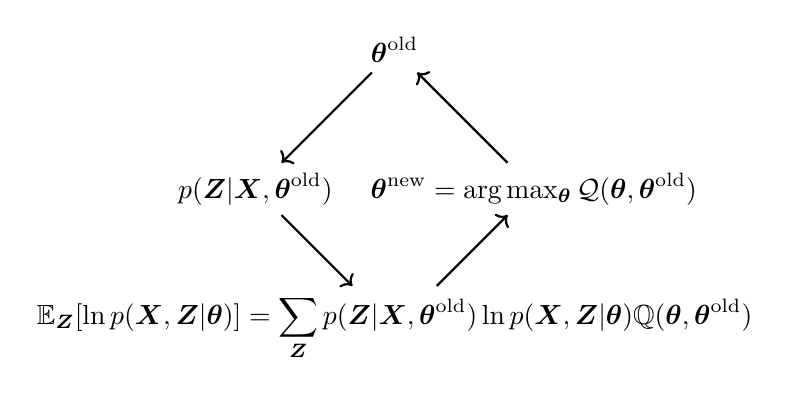
\begin{tikzpicture}[node distance=2.5cm]
\tikzstyle{arrow}=[->,thick];
\node (1) [] {$\btheta^\text{old}$};
\node (2) [below left of=1] {$p(\bZ|\bX,\btheta^\text{old})$};
\node (3) [below right of=2] {$\E_{\bZ}[\ln p(\bX,\bZ|\btheta)]=\displaystyle\sum_{\bZ}
p(\bZ|\bX,\btheta^\text{old})\ln p(\bX,\bZ|\btheta)\Q (\btheta,\btheta^\text{old})$};
\node (4) [below right of=1] {$\btheta^\text{new}=\text{arg} \max_{\btheta}\calq(\btheta,\btheta^\text{old})$};
\draw [arrow] (1) -- (2);
\draw [arrow] (2) -- (3);
\draw [arrow] (3) -- (4);
\draw [arrow] (4) -- (1);
\end{tikzpicture}
\section{reinforcement learning}
\label{sec:org82fcd40}

\section{wef}
\label{sec:orgae94296}
\subsection{wfe}
\label{sec:org9756ee4}
K-means
\end{document}